\documentclass[12pt,a4paper]{report}
% -------------------------------------------------------------------- %
% Pacotes

\usepackage[utf8]{inputenc}
\usepackage[T1]{fontenc}
\usepackage[brazil]{babel}
\usepackage[fixlanguage]{babelbib}
\usepackage[pdftex]{graphicx}      % usamos arquivos pdf/png como figuras
\usepackage{setspace}              % espaçamento flexvel
\usepackage{indentfirst}           % indentação do primeiro parágrafo
\usepackage{makeidx}               % índice remissivo
\usepackage[nottoc]{tocbibind}     % acrescentamos a bibliografia/indice/conteudo no Table of Contents
\usepackage{courier}               % usa o Adobe Courier no lugar de Computer Modern Typewriter
\usepackage{type1cm}               % fontes realmente escaláveis
\usepackage{titletoc}
\usepackage{ucs}
\usepackage[font=small,format=plain,labelfont=bf,up,textfont=it,up]{caption}
\usepackage[usenames,svgnames,dvipsnames]{xcolor}
\usepackage[a4paper,top=2.54cm,bottom=2.0cm,left=2.0cm,right=2.54cm]{geometry} % margens
\usepackage{amsmath} 

\usepackage[pdftex,plainpages=false,pdfpagelabels,pagebackref,colorlinks=true,citecolor=DarkGreen,
linkcolor=Black,urlcolor=Blue,filecolor=green,bookmarksopen=true]{hyperref} % links coloridos
\usepackage[all]{hypcap}                % soluciona o problema com o hyperref e capítulos
\usepackage[square,sort,nonamebreak,comma]{natbib}  % citação bibliográfica alpha
\fontsize{60}{62}\usefont{OT1}{cmr}{m}{n}{\selectfont}
\usepackage{upquote}                    % formata apóstrofes '
\usepackage{textcomp}

% Para formatar corretamente as URLs
\usepackage{url}
% -------------------------------------------------------------------- %
% Cabeçalhos similares ao TAOCP de Donald E. Knuth
\usepackage{fancyhdr}
\pagestyle{fancy}
\fancyhf{}
\renewcommand{\chaptermark}[1]{\markboth{\MakeUppercase{#1}}{}}
\renewcommand{\sectionmark}[1]{\markright{\MakeUppercase{#1}}{}}
\renewcommand{\headrulewidth}{0pt}

% -------------------------------------------------------------------- %
\graphicspath{{./imagens/}}        % caminho das figuras
\frenchspacing                     % arruma o espaço: id est (i.e.) e exempli gratia (e.g.)
\urlstyle{same}                    % URL com o mesmo estilo do texto e no mono-spaced
\makeindex                         % para o índice remissivo
\raggedbottom                      % para no permitir espaços extras no texto
\fontsize{60}{62}\usefont{OT1}{cmr}{m}{n}{\selectfont}
\cleardoublepage
\normalsize

% -------------------------------------------------------------------- %
% Cores para formatação de código
\usepackage{color}
\definecolor{vermelho}{rgb}{0.6,0,0} % para strings
\definecolor{verde}{rgb}{0.25,0.5,0.35} % para comentários
\definecolor{roxo}{rgb}{0.5,0,0.35} % para palavras-chaves
\definecolor{azul}{rgb}{0.25,0.35,0.75} % para strings
\definecolor{cinza-claro}{gray}{0.95}
% -------------------------------------------------------------------- %
% Opções de listagem usados para o código fonte
% Ref: http://en.wikibooks.org/wiki/LaTeX/Packages/Listings



\usepackage{listings}           % para formatar código-fonte (ex. em Java)


\lstset{ %
language=[Objective]Caml,  % seleciona a linguagem do código (aqui em lstlang0.sty
basicstyle=\footnotesize\ttfamily, % o tamanho da fonte usado no código
commentstyle=\color{verde}\bfseries,  % formatação de comentários
stringstyle=\color{azul},    % formatação de strings
upquote=true,
numbers=left,                   % onde colocar os números de linha
numberstyle=\tiny,  % o tamanho da fonte usada para a numeração das linhas
stepnumber=1,                   % o intervalo entre dois números de linhas. Se for 1, numera cada uma.
numbersep=5pt,                  % how far the line-numbers are from the code
showspaces=false,               % show spaces adding particular underscores
showstringspaces=false,         % underline spaces within strings
showtabs=false,                 % show tabs within strings adding particular underscores
keywordstyle=\color{roxo}\bfseries,
keywordstyle=[1]\color{roxo}\bfseries,
keywordstyle=[2]\color{verde}\bfseries,
%        keywordstyle=[3]\textbf,    %
%        keywordstyle=[4]\textbf,   \sqrt{\sqrt{}} %
frame=b,                   % adds a frame around the code
framerule=0.6pt,
tabsize=2,                      % sets default tabsize to 2 spaces
captionpos=t,                   % sets the caption-position to top
breaklines=true,                % sets automatic line breaking
breakatwhitespace=false,        % sets if automatic breaks should only happen at whitespace
escapeinside={\%*}{*)},         % if you want to add a comment within your code
backgroundcolor=\color[rgb]{0.93,0.93,0.92}, % choose the background color.
rulecolor=\color[rgb]{0.8,0.8,0.8},
extendedchars=true,
xleftmargin=10pt,
xrightmargin=10pt,
framexleftmargin=10pt,
framexrightmargin=10pt,
literate={â}{{\^{a}}}1  % para formatar corretamente os acentos do Português ao usar utf8
    {ê}{{\^{e}}}1
    {ô}{{\^{o}}}1  
    {Â}{{\^{A}}}1
    {Ê}{{\^{E}}}1
    {Ô}{{\^{O}}}1
    {á}{{\'{a}}}1
    {é}{{\'{e}}}1
    {í}{{\'{i}}}1
    {ó}{{\'{o}}}1
    {ú}{{\'{u}}}1
    {Á}{{\'{A}}}1
    {É}{{\'{E}}}1
    {Í}{{\'{I}}}1
    {Ó}{{\'{O}}}1
    {Ú}{{\'{U}}}1
    {à}{{\`{a}}}1
    {À}{{\`{A}}}1
    {ã}{{\~{a}}}1
    {õ}{{\~{o}}}1
    {Ã}{{\~{A}}}1
    {Õ}{{\~{O}}}1
    {ç}{{\c{c}}}1
    {Ç}{{\c{C}}}1
    {ü}{{\"u}}1
    {Ü}{{\"U}}1
}

\renewcommand{\lstlistingname}{Programa}
\renewcommand{\lstlistlistingname}{Lista de Arquivo}

% Definição de novos estilos
\lstdefinestyle{Bash}
    {language=bash,frame=single,numbers=none,basicstyle=\footnotesize\ttfamily,
     morekeywords={cp,mkdir,sudo,tar}}

% Definição de novos ambientes
\lstnewenvironment{terminal}
  {\lstset{style=Bash}}
  {}

\lstnewenvironment{ocaml}
  {\lstset{basicstyle=\scriptsize\ttfamily,
           frame=single,
           frameround=tttt,
           framerule=2pt,
           numbers=none,
           rulecolor=\color{Salmon}}}
  {}

\lstnewenvironment{xml}
   {\lstset{language=XML,frame=single,numbers=none}}
   {}

\lstnewenvironment{interprete}
  {\lstset{frame=single,
            frameround=tttt,
            numbers=none,
            basicstyle=\ttfamily,
            framerule=2pt,
            rulecolor=\color{CadetBlue}}}
  {}
% Formata o caption da listagem
% \DeclareCaptionFont{blue}{\color{blue}} 

% \captionsetup[lstlisting]{singlelinecheck=false, labelfont={blue}, textfont={blue}}
\usepackage{caption}
\DeclareCaptionFont{white}{\color{white}}
\DeclareCaptionFormat{listing}{\colorbox[cmyk]{0.43, 0.35, 0.35,0.01}{\parbox{\textwidth}{\hspace{15pt}#1#2#3}}}
\captionsetup[lstlisting]{format=listing,labelfont=white,textfont=white, singlelinecheck=false, margin=0pt, font={bf,footnotesize}}

\newcommand{\ListingsPath}{./codigos}
% Inclui o nome do arquivo como Caption 
\newcommand{\filelisting}[2][]{%
    \lstinputlisting[caption={\texttt{\detokenize{#2}}},#1]{\ListingsPath/#2}%
}

% ---------------------------------------------------------------------------- %

% ---------------------------------------------------------------------------- %

\title{Construção de um Compilador para MiniLua usando Objective Caml}
\date{}
\author{Henrique Araújo Lima \\
\texttt{\small \url{henriquebrmg@gmail.com}}\\ \\
Vinicius Lopes da Silva Teixeira \\
\texttt{\small \url{viniciuslt@outlook.com}}\\ 
\vspace{1cm} \\
Faculdade de Computação \\
Universidade Federal de Uberlândia
}

\date{14 de dezembro de 2016}

%\includeonly{cap-clojure,magical,short}
\begin{document}
  \maketitle
% -------------------------------------------------------------------- %


% -------------------------------------------------------------------- %
% Sumário
\tableofcontents    


% Capítulos do trabalho


% cabeçalho para as páginas de todos os capítulos
%\fancyhead[RE,LO]{\thesection}

%\singlespacing              % espaçamento simples
\setlength{\parskip}{0.15in} % espaçamento entre paragráfos

\chapter{Introdução}
Este trabalho tem como objetivo construir um compilador da linguagem de programação Lua. Para esta construção utilizaremos a linguagem funcional OCaml.

\section{OCaml}
Objective Caml, também conhecida como OCaml (Ojective Categorical Abstract Machine Language), é uma linguagem de programação funcional da família ML, desenvolvida pelo INRIA em 1996. Trata-se da linguagem Caml com a adição de suporte de técnicas de orientação a objetos e algumas alterações e extensões de sintaxe.

\subsection{Instalação}
O comando para instalar o Ocaml no Ubuntu 16.04 é:
\begin{terminal}
> sudo apt-get install ocaml
\end{terminal}

\section{CRL}
A Common Language Runtime (CLR), um componente da máquina virtual do framework Microsoft .NET que gerencia a execução de programas .NET. Um processo de compilação conhecido por just-in-time que converte o código compilado em instruções de máquina ao qual a CPU do computador executa.

\section{CIL}

O Common Intermediate Language (CLI) descreve o código executável e o ambiente de execução que formam o núcleo do Framework .NET da Microsoft, do MONO e do Portable.NET, sendo as duas últimas implementações gratuitas e de código aberto da mesma. A Common Language Runtime é a implementação da CLI pela Microsoft, em outras palavras, é uma máquina virtual que segue um padrão internacional e a base para a criação e execução de ambientes de desenvolvimento em que as linguagens e as bibliotecas trabalham juntos.


\subsection{Instruções}
A lista do conjunto de instruções do CLI podem ser encontradas em: \url{https://en.wikipedia.org/wiki/List_of_CIL_instructions}

\subsection{Compilação}
O comando para compilar um arquivo é :
\begin{terminal}
> ilasm "nome_do_arquivo".il
\end{terminal}
É necessário que o arquivo tenha extensão ".il"

\subsection{Execução}
O comando para executar um arquivo é :
\begin{terminal}
> mono "nome_do_arquivo".exe
\end{terminal}
É necessário que o arquivo tenha extensão ".exe"



\section{Mono}
O Mono é um projeto liderado pela Novell (anteriormente pela Ximian) para criar um conjunto de ferramentas compatíveis com a plataforma .NET, conforme as normas ECMA, incluindo, entre outras, um compilador C Sharp e um CLR. O principal objetivo do Mono não é somente ser capaz de rodar aplicações .NET multi-plataformas, mas também proporcionar melhores ferramentas de desenvolvimento para desenvolvedores Linux.

\subsection{Instalação}
O comando para instalar o Mono no Ubuntu 16.04 é:
\begin{terminal}
> sudo apt-get install mono-complete
\end{terminal}


\chapter{Programas}
Todos os programas com extensão ".il" ou seja os assemblys foram gerados "na mão", com exceção do programa descrito na seção 2.13 onde foi utilizado um programa escrito em C\# para gerar o correspondente em assembly.  

\section{Módulo Mínimo}
MiniLua
\lstinputlisting[caption={nano01.lua}]{codigos/nano01.lua}

CIL
\lstinputlisting[caption={nano01.il}]{codigos/CIL/nano01.il}



\section{Declaração de uma variável}
 MiniLua
\lstinputlisting[caption={nano02.il}]{codigos/nano02.lua}

CIL
\lstinputlisting[caption={nano02.il}]{codigos/CIL/nano02.il}



\section{Atribuição de um inteiro a uma variável }

MiniLua
\lstinputlisting[caption={nano03.lua}]{codigos/nano03.lua}

CIL
\lstinputlisting[caption={nano03.il}]{codigos/CIL/nano03.il}



\section{Atribuição de uma soma de inteiros a uma variável }
MiniLua
\lstinputlisting[caption={nano04.lua}]{codigos/nano04.lua}

CIL
\lstinputlisting[caption={nano04.il}]{codigos/CIL/nano04.il}



\section{Inclusão do comando de impressão }
MiniLua
\lstinputlisting[caption={nano05.lua}]{codigos/nano05.lua}

CIL
\lstinputlisting[caption={nano05.il}]{codigos/CIL/nano05.il}



\section{Atribuição de uma subtração de inteiros a uma variável }
 MiniLua
\lstinputlisting[caption={nano06.lua}]{codigos/nano06.lua}

CIL
\lstinputlisting[caption={nano06.il}]{codigos/CIL/nano06.il}



\section{Inclusão do comando condicional }
 MiniLua
\lstinputlisting[caption={nano07.lua}]{codigos/nano07.lua}

CIL
\lstinputlisting[caption={nano07.il}]{codigos/CIL/nano07.il}



\section{Inclusão do comando condicional com parte senão }
 MiniLua
\lstinputlisting[caption={nano08.lua}]{codigos/nano08.lua}

CIL
\lstinputlisting[caption={nano08.il}]{codigos/CIL/nano08.il}



\section{Atribuição de duas operações aritméticas sobre inteiro a uma variável }
MiniLua
\lstinputlisting[caption={nano09.lua}]{codigos/nano09.lua}

CIL
\lstinputlisting[caption={nano09.il}]{codigos/CIL/nano09.il}



\section{Atribuição de duas variáveis inteiras }
MiniLua
\lstinputlisting[caption={nano10.lua}]{codigos/nano10.lua}

CIL
\lstinputlisting[caption={nano10.il}]{codigos/CIL/nano10.il}



\section{Atribuição de um comando de repetição enquanto }
MiniLua
\lstinputlisting[caption={nano11.lua}]{codigos/nano11.lua}

CIL
\lstinputlisting[caption={nano11.il}]{codigos/CIL/nano11.il}



\section{Comando condicional aninhado em um comando de repetição}
MiniLua
\lstinputlisting[caption={nano12.lua}]{codigos/nano12.lua}

CIL
\lstinputlisting[caption={nano12.il}]{codigos/CIL/nano12.il}


\section{Converte graus Celsius para Fahrenheit }
MiniLua
\lstinputlisting[caption={micro01.lua}]{codigos/micro01.lua}

C\#
\lstinputlisting[caption={micro01.cs}]{codigos/micro01.cs}

Para gerar o arquivo "micro01.il" a partir do programa "micro01.cs" em C\#, foram executados os seguintes comandos:

\begin{terminal}
> mcs micro01.cs
> monodis micro01.exe > micro01.il
\end{terminal}

CIL
\lstinputlisting[caption={micro01.il \label{arq:micro01}}]{codigos/CIL/micro01.il}


Para compilar e executar o arquivo "micro01.il" foram feitos os seguintes comandos:

\begin{terminal}
> ilasm micro01.il
> mono micro01.exe
\end{terminal}



\section{Decide qual maior }
MiniLua
\lstinputlisting[caption={micro02.lua}]{codigos/micro02.lua}
CIL
\lstinputlisting[caption={micro02.il}]{codigos/CIL/micro02.il}



\section{Le o número e verifica se está entre 100 e 200 }
MiniLua
\lstinputlisting[caption={micro03.lua}]{codigos/micro03.lua}
CIL
\lstinputlisting[caption={micro03.il}]{codigos/CIL/micro03.il}



\section{Le números e informa quais estão entre 10 e 150 }
MiniLua
\lstinputlisting[caption={micro04.lua}]{codigos/micro04.lua}
CIL
\lstinputlisting[caption={micro04.il}]{codigos/CIL/micro04.il}



\section{Le strings e caracteres }
MiniLua
\lstinputlisting[caption={micro05.lua}]{codigos/micro05.lua}
CIL
\lstinputlisting[caption={micro05.il}]{codigos/CIL/micro05.il}



\section{Escreve um número lido por extenso }
MiniLua
\lstinputlisting[caption={micro06.lua}]{codigos/micro06.lua}
CIL
\lstinputlisting[caption={micro06.il}]{codigos/CIL/micro06.il}



\section{Decide se os números são positivos, negativos ou zero }
MiniLua
\lstinputlisting[caption={micro07.lua}]{codigos/micro07.lua}
CIL
\lstinputlisting[caption={micro07.il}]{codigos/CIL/micro07.il}



\section{Decide se um número é maior que 10 }
MiniLua
\lstinputlisting[caption={micro08.lua}]{codigos/micro08.lua}
CIL
\lstinputlisting[caption={micro08.il}]{codigos/CIL/micro08.il}



\section{Cálculo de preços}
MiniLua
\lstinputlisting[caption={micro09.lua}]{codigos/micro09.lua}
CIL
\lstinputlisting[caption={micro09.il}]{codigos/CIL/micro09.il}



\section{Calcula o fatorial de um número}
MiniLua
\lstinputlisting[caption={micro10.lua}]{codigos/micro10.lua}
CIL
\lstinputlisting[caption={micro10.il}]{codigos/CIL/micro10.il}



\section{Decide se um numero é positivo, zero ou negativo com auxılio de uma função}
MiniLua
\lstinputlisting[caption={micro11.lua\label{arq:micro11}}]{codigos/micro11.lua}
CIL
\lstinputlisting[caption={micro11.il}]{codigos/CIL/micro11.il}


\chapter{Construindo o Compilador}

\section{Analisador Léxico}
Análise léxica é o processo de analisar a entrada de linhas de caracteres e produzir uma seqüência de símbolos chamado "símbolos léxicos", ou somente "símbolos" (tokens). O componente do compilador responsável pela execução desse processo é conhecido como Analisador léxico.

O analisador léxico, faz a varredura do programa fonte caractere por caractere e, traduz em uma seqüência de símbolos léxicos ou tokens. É nessa fase que são reconhecidas as palavras reservadas, constantes, identificadores e outras palavras que pertencem a linguagem de programação. O analisador léxico executas outras tarefas como por exemplo o tratamento de espaços, eliminação de comentários, contagem do número de linhas que o programa possui e etc.

\subsection{Analisador Léxico Manual para Pascal}
Abaixo temos um analisador léxico feito manualmente.
\lstinputlisting[caption={dfalexer.ml \label{arq:dfalexer}}]{codigos/Lexer/dfalexer.ml}

\subsubsection{Como Usar}

Para testar o analisador léxico utilizaremos dos seguintes comandos:
\begin{terminal}
> rlwrap ocaml
# #use "nome_do_arquivo.ml";;
# lexico "cadeia de strings";;
\end{terminal}

\subsubsection{Estrutura do Analisador Léxico}

\begin{figure}[!htb]
\centering
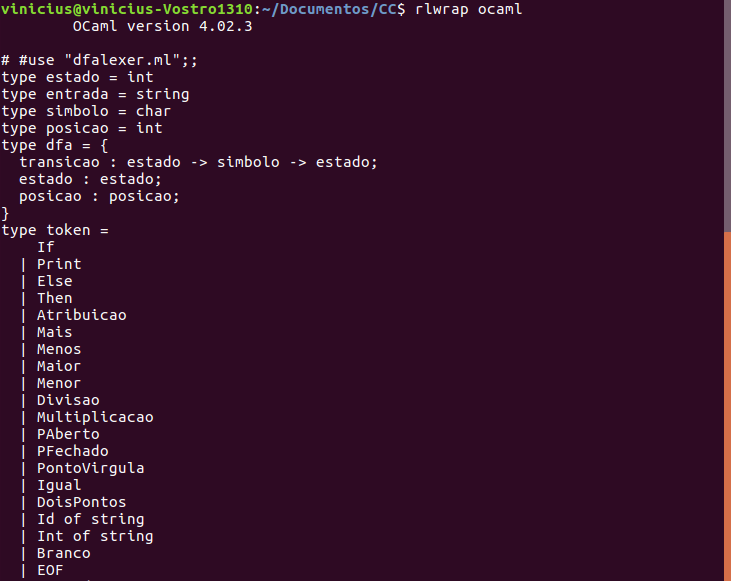
\includegraphics[scale=0.6]{Imagens/img1.png}
\caption{Estrutura do Analisador(1)}
\label{img1}
\end{figure}

\begin{figure}[!htb]
\centering
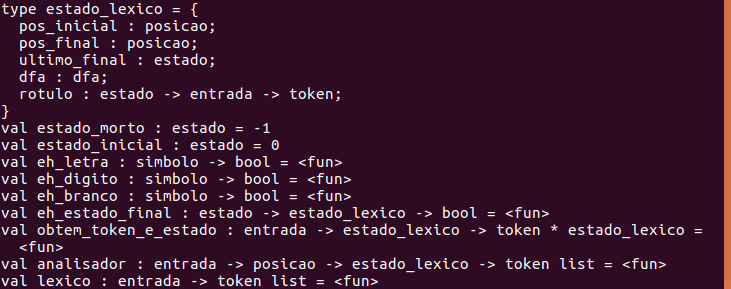
\includegraphics[scale=0.6]{Imagens/img2.png}
\caption{Estrutura do Analisador(2)}
\label{img2}
\end{figure}

\subsubsection{Exemplos}
Veremos alguns exemplos para um analisador da linguagem Pascal.

\begin{figure}[!htb]
\centering

\includegraphics[scale=0.6]{Imagens/img4.png}
\caption{print (a * b);}
\label{img4}
\end{figure}

\begin{figure}[!htb]
\centering

\includegraphics[scale=0.6]{Imagens/img5.png}
\caption{if1 := a - 2;}
\label{img5}
\end{figure}

\begin{figure}[!htb]
\centering

\includegraphics[scale=0.6]{Imagens/img6.png}
\caption{if if1 > 0}
\label{img6}
\end{figure}

\begin{figure}[!htb]
\centering
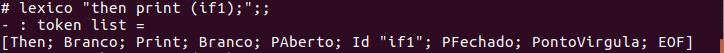
\includegraphics[scale=0.6]{Imagens/img7.png}
\caption{then print (if1);}
\label{img7}
\end{figure}

\begin{figure}[!htb]
\centering

\includegraphics[scale=0.6]{Imagens/img9.png}
\caption{else @print (if2);}
\label{img9}
\end{figure}


\subsection{Analisador Léxico Automático para Lua}

Lua é uma linguagem de formato livre. Ela ignora espaços (incluindo quebras de linha) e comentários entre elementos léxicos (tokens), exceto como delimitadores entre nomes e palavras-chave.

Nomes (também chamados de identificadores) em Lua podem ser qualquer cadeia de letras, dígitos, e sublinhados, que não iniciam com um dígito. 

No programa a seguir serão implementadas as palavras reservadas da linguagem Lua, ou seja, as palavras que não podem ser usadas como nomes, e também as demais regras da linguagem, tais como tratamento de comentários e strings. 

\lstinputlisting[caption={lexico.mll \label{arq:lexico}}]{codigos/Lexer/lexico.mll}

\subsubsection{Carregador}

Também é necessario o uso de um carregador para fazer load dos arqivos ".cmo" e para pegar a entrada por arquivo ou por uma string.

\lstinputlisting[caption={carregador.ml \label{arq:carregador}}]{codigos/Lexer/carregador.ml}


\subsubsection{Compilando}

Para compilar o analisador léxico de Lua utilizaremos dos seguintes comandos:

\begin{terminal}
> ocamllex lexico.mll
\end{terminal}
Após este comando sera gerado um arquivo de nome "lexico.ml" que sera usado no proximo comando.

\begin{terminal}
> ocamc -c lexico.ml
\end{terminal}

Pode-se verificar que após este comando serão criados dois arquivos, um chamado "lexico.cmi" e outro com nome "lexico.cmo".


\subsubsection{Testando}

Para testar o analisador léxico utilizaremos dos seguintes comandos:

\begin{terminal}
> rlwrap ocaml
# #use "carregador.ml";;
# lex "arquivo.lua";;
\end{terminal}

\subsubsection{Exemplo}

O seguinte programa será utilizado como exemplo:

\lstinputlisting[caption={micro03.lua }]{codigos/micro03.lua}

e produzirá uma saida com os seguintes tokens:

\begin{figure}[!htb]
\centering
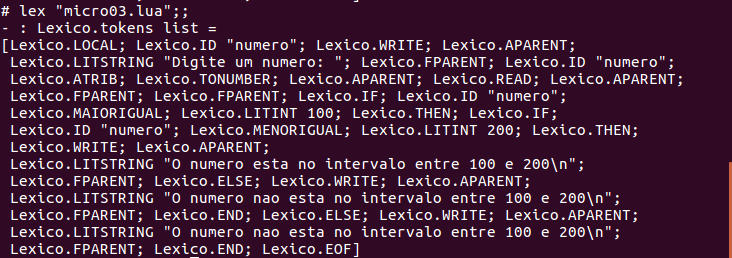
\includegraphics[scale=0.64]{Imagens/img10.png}
\caption{saída do analisador léxico}
\label{img10}
\end{figure}

\section{Analisador sintático}

Análise sintática é o processo de analisar uma sequência de entrada para determinar sua estrutura gramatical segundo uma determinada gramática formal.
A análise sintática transforma um texto na entrada em uma estrutura de dados, em geral uma árvore, o que é conveniente para processamento posterior e captura a hierarquia implícita desta entrada. Através da análise léxica é obtido um grupo de tokens, para que o analisador sintático use um conjunto de regras para construir uma árvore sintática da estrutura.


\subsection{Parser preditivo}

Construindo um parser preditivo para a gramatica a seguir:
\begin{figure}[!htb]
\centering
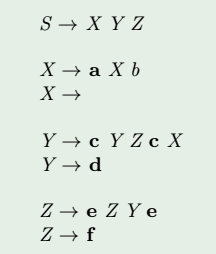
\includegraphics[scale=0.7]{Imagens/parser.png}
\caption{gramatica para gerar o parser}
\label{parser}
\end{figure}

\lstinputlisting[caption={parserlexico }]{codigos/Parser/lexico.mll}

\lstinputlisting[caption={parsersintatico }]{codigos/Parser/sintatico.mli}

\lstinputlisting[caption={parserarv }]{codigos/Parser/sintaticoArv.ml}

\subsubsection{Compilar}

Para compilar deve-se realizar os seguintes comandos:
\begin{terminal}
> ocamllex lexico.mll
> ocaml -c sintatico.mli
> ocaml -c lexico.ml
\end{terminal}


\subsubsection{Testar}

Para testar serão utilizados os seguintes comandos:

\begin{terminal}
> rlwrap ocaml
# #use "sintaticoArv.ml";;
# teste();;
\end{terminal}

\subsubsection{Exemplo}

Como pode ser observado ma linha 97 do \textbf{Programa 3.7}, será utilizada a palavra "abcdfcf" para verificar se esta pertence a linguagem gerada pela gramática descrita na \textbf{figura 3.9}

\begin{figure}[!htb]
\centering
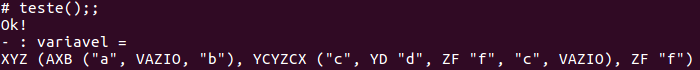
\includegraphics[scale=0.64]{Imagens/teste.png}
\caption{testando o parser}
\label{teste}
\end{figure}

Além de verificar se a palavra pertence a linguagem, a função "teste()" nos mostra a árvore sintática gerada neste problema. 



\subsection{Analisador sintático com mensagens de erros}

Nesta subseção será criado um analisador sintático abstrato completo para a linguagem Lua.

Primeiramente os seguintes comandos devem ser executados para a instalação do "opam" e do "menhir":

\begin{terminal}
> sudo apt install opam
> opam init
> eval `opam config env`
> sudo apt-get install m4
> opam install menhir
\end{terminal}


\subsubsection{Criando os arquivos iniciais}

\lstinputlisting[caption={Analisador - lexico.mll}]{codigos/Analisador_Sint/lexico.mll}

\lstinputlisting[caption={Analisador - ast.ml}]{codigos/Analisador_Sint/ast.ml}

\lstinputlisting[caption={Analisador - sintatico.mly}]{codigos/Analisador_Sint/sintatico.mly}

\lstinputlisting[caption={Analisador - sintaticoTest.ml}]{codigos/Analisador_Sint/sintaticoTest.ml}


\subsubsection{Gerando as mensagens de erro}
\label{errosint}
Após criarmos os arquivos iniciais, as mensagens de erro devem ser geradas.
Foi executado no terminal:

\begin{terminal}
> menhir -v --list-errors sintatico.mly > sintatico.msg
\end{terminal}

Após a execução um arquivo chamado "sintatico.msg" foi criado. Este arquivo foi modificado da seguinte maneira: onde tinha a string "<YOUR SYNTAX ERROR MESSAGE HERE>" foi passado para ``Esperava um bloco de comandos'' por exemplo.


Depois o seguinte comando foi executado:

\begin{terminal}
> menhir -v --list-errors sintatico.mly --compile-errors sintatico.msg > erroSint.ml
\end{terminal}


\subsubsection{Criando o carregador}

O seguinte carregador foi criado com o nome de ``.ocamlinit''. 

\lstinputlisting[caption={Analisador - .ocamlinit}]{codigos/Analisador_Sint/ocamlinit.txt}


\subsubsection{Compilando}

Para compilar, o seguinte comando foi executado:

\begin{terminal}
> ocamlbuild -use-ocamlfind -use-menhir -menhir "menhir --table" -package menhirLib sintaticoTest.byte
\end{terminal}

\subsubsection{Testando}

Será testado o seguinte arquivo:

\lstinputlisting[caption={micro11.lua }]{codigos/micro11.lua}


Para testar deve-se entrar no ocaml assim:

\begin{terminal}
> rlwrap ocaml
\end{terminal}

Depois digitar no terminal:

\begin{terminal}
> parse_arq "micro11.lua";;
\end{terminal}

O retorno deste comando será:

\begin{figure}[!htb]
\centering
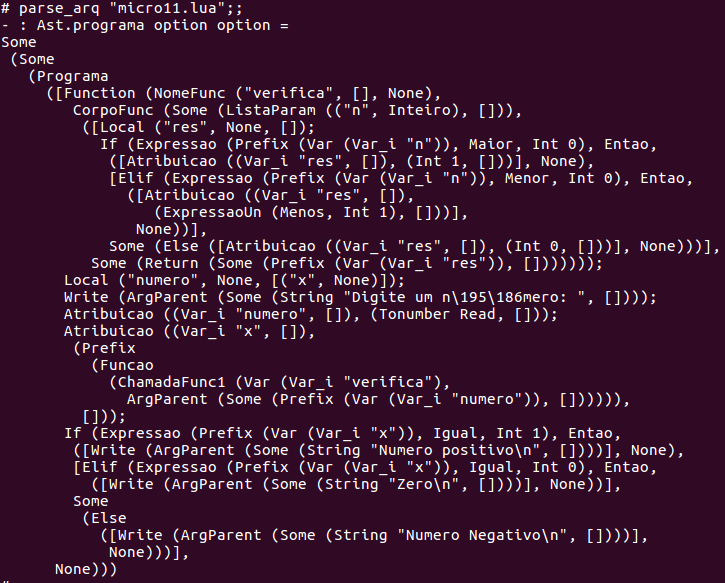
\includegraphics[scale=0.64]{Imagens/arvoremicro11.png}
\caption{Árvore sintática abstrata}
\label{arvoremicro11}
\end{figure}


\section{Analisador Semântico}

Algumas alerações foram feitas nos arquivos ``lexico.mll'', ``ast.ml'' e ``sintatico.mly'' da análise sintática, como pode ser visto a seguir:

\lstinputlisting[caption={Analisador Semântico - lexico.mll}]{codigos/Analisador_Seman/lexico.mll}

\lstinputlisting[caption={Analisador Semântico - ast.ml}]{codigos/Analisador_Seman/ast.ml}

\lstinputlisting[caption={Analisador Semântico - sintatico.mly}]{codigos/Analisador_Seman/sintatico.mly}

Consequentemente as mensagens de erro também foram atualizadas seguindo os passos indicados em \ref{errosint}.


\subsection{Criando os arquivos semânticos}

O seguinte arquivo foi criado com o nome de ``semantico.ml''

\lstinputlisting[caption={Analisador Semântico - semantico.ml}]{codigos/Analisador_Seman/semantico.ml}

Depois foi criado o ``ambiente.ml'':

\lstinputlisting[caption={Analisador Semântico - ambiente.ml}]{codigos/Analisador_Seman/ambiente.ml}


Também foram criados o ``sast.ml'' e o ``tast.ml'', mostrados a seguir:

\lstinputlisting[caption={Analisador Semântico - sast.ml}]{codigos/Analisador_Seman/sast.ml}

\lstinputlisting[caption={Analisador Semântico - tast.ml}]{codigos/Analisador_Seman/tast.ml}


\subsection{Compilando}

Para compilar, primeiramente é necessario criar o arquivo ``semanticoTest.ml'':

\lstinputlisting[caption={Analisador Semântico - semanticoTest.ml}]{codigos/Analisador_Seman/semanticoTest.ml}

Agora deve-se digitar no terminal: 

\begin{terminal}
> ocamlbuild -use-ocamlfind -use-menhir -menhir "menhir --table" -package menhirLib semanticoTest.byte
\end{terminal}

\subsection{Testando}

Será testado o seguinte arquivo:

\lstinputlisting[caption={micro10.lua }]{codigos/Analisador_Seman/micro10.lua}


Para testar deve-se entrar no ocaml assim:

\begin{terminal}
> rlwrap ocaml
\end{terminal}

Depois digitar no terminal:

\begin{terminal}
> verifica_tipos "micro10.lua";;
\end{terminal}

O retorno deste comando será a seguinte árvore tipada:

\lstinputlisting[caption={Analisador Semântico - retorno}]{codigos/Analisador_Seman/retorno_micro10.txt}


\section{Interpretador}

A ultima etapa foi fazer um interpretador para miniLua, seguindo os seguintes passos:

A tabela de simbolos com mome de ``tabsimb.ml'' foi criada da seguinte maneira:

\lstinputlisting[caption={Interpretador - tabsimb.ml}]{codigos/Interpretador/tabsimb.ml}

Depois foi criado o ambiente do interpretador, que é diferente do ambiente semantico, com o nome de ``ambInterp.ml'':

\lstinputlisting[caption={Interpretador - ambInterp.ml}]{codigos/Interpretador/ambInterp.ml}

O ultimo passo foi criar o interpretador, nomeado de ``interprete.ml'':

\lstinputlisting[caption={Interpretador - interprete.ml}]{codigos/Interpretador/interprete.ml}



\subsection{Compilando}

Para compilar, primeiramente é necessario criar o arquivo ``interpreteTeste.ml'':

\lstinputlisting[caption={Interpretador - interpreteTeste.ml}]{codigos/Interpretador/interpreteTeste.ml}

Agora deve-se digitar no terminal: 

\begin{terminal}
> ocamlbuild -use-ocamlfind -use-menhir -menhir "menhir --table" -package menhirLib interpreteTeste.byte
\end{terminal}

\subsection{Testando}

Será testado o seguinte arquivo:

\lstinputlisting[caption={micro10.lua }]{codigos/Analisador_Seman/micro10.lua}


Para testar deve-se entrar no ocaml assim:

\begin{terminal}
> rlwrap ocaml
\end{terminal}

Depois digitar no terminal:

\begin{terminal}
> interprete "micro10.lua";;
\end{terminal}

O retorno deste comando será:

\begin{figure}[!htb]
\centering
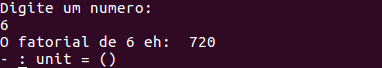
\includegraphics[scale=0.9]{codigos/Interpretador/fat.png}
\caption{Interpretador: Fatorial}
\label{fatorial}
\end{figure}


\end{document} 
